\documentclass{sig-alternate}

\usepackage{epstopdf}
\usepackage{float}
\usepackage{graphicx}


\begin{document}

% Copyright
%\setcopyright{acmcopyright}
%\setcopyright{acmlicensed}
%\setcopyright{rightsretained}
%\setcopyright{usgov}
%\setcopyright{usgovmixed}
%\setcopyright{cagov}
%\setcopyright{cagovmixed}


% DOI
%\doi{10.475/123_4}

% ISBN
%\isbn{123-4567-24-567/08/06}

%Conference
%\conferenceinfo{PLDI '13}{June 16--19, 2013, Seattle, WA, USA}

%\acmPrice{\$15.00}

%
% --- Author Metadata here ---
%\conferenceinfo{WOODSTOCK}{'97 El Paso, Texas USA}
%\CopyrightYear{2007} % Allows default copyright year (20XX) to be over-ridden - IF NEED BE.
%\crdata{0-12345-67-8/90/01}  % Allows default copyright data (0-89791-88-6/97/05) to be over-ridden - IF NEED BE.
% --- End of Author Metadata ---

\title{Automatic Labelling of Videos using Deep Neural Network}
\subtitle{CSE 847 Project Proposal}
%\titlenote{A full version of this paper is available as
%\textit{Author's Guide to Preparing ACM SIG Proceedings Using
%\LaTeX$2_\epsilon$\ and BibTeX} at
%\texttt{www.acm.org/eaddress.htm}}}
%
% You need the command \numberofauthors to handle the 'placement
% and alignment' of the authors beneath the title.
%
% For aesthetic reasons, we recommend 'three authors at a time'
% i.e. three 'name/affiliation blocks' be placed beneath the title.
%
% NOTE: You are NOT restricted in how many 'rows' of
% "name/affiliations" may appear. We just ask that you restrict
% the number of 'columns' to three.
%
% Because of the available 'opening page real-estate'
% we ask you to refrain from putting more than six authors
% (two rows with three columns) beneath the article title.
% More than six makes the first-page appear very cluttered indeed.
%
% Use the \alignauthor commands to handle the names
% and affiliations for an 'aesthetic maximum' of six authors.
% Add names, affiliations, addresses for
% the seventh etc. author(s) as the argument for the
% \additionalauthors command.
% These 'additional authors' will be output/set for you
% without further effort on your part as the last section in
% the body of your article BEFORE References or any Appendices.

\numberofauthors{2} %  in this sample file, there are a *total*
% of EIGHT authors. SIX appear on the 'first-page' (for formatting
% reasons) and the remaining two appear in the \additionalauthors section.
%
\author{
% You can go ahead and credit any number of authors here,
% e.g. one 'row of three' or two rows (consisting of one row of three
% and a second row of one, two or three).
%
% The command \alignauthor (no curly braces needed) should
% precede each author name, affiliation/snail-mail address and
% e-mail address. Additionally, tag each line of
% affiliation/address with \affaddr, and tag the
% e-mail address with \email.
%
% 1st. author
\alignauthor
Tarang Chugh\\
       \email{chughtar@msu.edu}
% 2nd. author
\alignauthor
Rahul Dey\\
       \email{deyrahul@msu.edu}
}
% There's nothing stopping you putting the seventh, eighth, etc.
% author on the opening page (as the 'third row') but we ask,
% for aesthetic reasons that you place these 'additional authors'
% in the \additional authors block, viz.
%\additionalauthors{Additional authors: John Smith (The Th{\o}rv{\"a}ld Group,
%email: {\texttt{jsmith@affiliation.org}}) and Julius P.~Kumquat
%(The Kumquat Consortium, email: {\texttt{jpkumquat@consortium.net}}).}
%\date{30 July 1999}
% Just remember to make sure that the TOTAL number of authors
% is the number that will appear on the first page PLUS the
% number that will appear in the \additionalauthors section.

\maketitle
%\begin{abstract}
%Abstract goes here.
%\end{abstract}


%
% The code below should be generated by the tool at
% http://dl.acm.org/ccs.cfm
% Please copy and paste the code instead of the example below. 
%
%\begin{CCSXML}
%<ccs2012>
% <concept>
%  <concept_id>10010520.10010553.10010562</concept_id>
%  <concept_desc>Computer systems organization~Embedded systems</concept_desc>
%  <concept_significance>500</concept_significance>
% </concept>
% <concept>
%  <concept_id>10010520.10010575.10010755</concept_id>
%  <concept_desc>Computer systems organization~Redundancy</concept_desc>
%  <concept_significance>300</concept_significance>
% </concept>
% <concept>
%  <concept_id>10010520.10010553.10010554</concept_id>
%  <concept_desc>Computer systems organization~Robotics</concept_desc>
%  <concept_significance>100</concept_significance>
% </concept>
% <concept>
%  <concept_id>10003033.10003083.10003095</concept_id>
%  <concept_desc>Networks~Network reliability</concept_desc>
%  <concept_significance>100</concept_significance>
% </concept>
%</ccs2012>  
%\end{CCSXML}

%\ccsdesc[500]{Computer systems organization~Embedded systems}
%\ccsdesc[300]{Computer systems organization~Redundancy}
%\ccsdesc{Computer systems organization~Robotics}
%\ccsdesc[100]{Networks~Network reliability}


%
% End generated code
%

%
%  Use this command to print the description
%
%\printccsdesc

% We no longer use \terms command
%\terms{Theory}

%\keywords{ACM proceedings; \LaTeX; text tagging}

\section{Problem Description}
In the last decade, the world wide web has witnessed a massive explosion of multimedia data due to the rise of online media-sharing services such as Youtube, Facebook, etc. While many studies have tackled the problem of analyzing and understanding static images~\cite{krizhevsky2012imagenet}, improvements in video understanding research has been lagging due to unavailability of large-scale labelled dataset. However, analysis and understanding of video content on these video-sharing services provide insights to make the interface more engaging and customized to individual needs. Relevant search results, improved video recommendations, and content filtering are some of the many desired properties, which require the understanding of video content. In this project, we aim to analyze and understand video content to accurately assign labels. Google's recent release of the Youtube-8M dataset accompanied~\cite{abu2016youtube} with the launch of the Kaggle competition\footnote{\url{https://www.kaggle.com/c/youtube8m}} to benchmark the performance on this task, has motivated us to take up this arduous task. We plan to take a deep learning based approach to design the classifier. We will also make use of the Google Cloud Machine Learning beta platform\footnote{\url{https://cloud.google.com/ml/}} available to the participants of this competition.

\section{Survey}
Convolutional Neural Networks (CNN) have emerged as a powerful tool for image based automation tasks such as recognition, segmentation, enhancement, encoding etc. It has become the preferred choice for such tasks as compared to other machine learning algorithms such as SVM, k-NN, Multilayer Neural Networks, etc. because of their unique ability to extract useful features from two dimensional inputs. However, when it comes to spatio-temporal inputs such as videos, CNN in itself is often found to be performing poorly. In our survey, we came across several approaches adopted by researchers to perform tasks such as video classification and labelling. We will discuss some of the approaches here briefly.

In case of videos, traditional CNN architectures suffer due to three main issues. The first issue relates to the large amount of computational resources required to train a CNN for classifying videos. For instance, videos of frame size $178 \times 178$, takes weeks to train a CNN using powerful GPUs. Performance of a deep neural network relies on the abundance of data. Thus, in case of videos, the size of data becomes even more, because of their three dimensional (two spatial and one temporal) nature. The second main issue is that CNN doesn't have any inbuilt mechanism to learn temporal patterns in the input data. And lastly, videos are usually of varying time duration. Even if all the input videos are resized to a particular resolution, different durations make them harder to be fed to a predesigned fixed network.

Several researchers have taken different approaches to overcome some of these issues. Karpathy et al.~\cite{karpathy2014large} suggested an approach where the input video is divided into two separate streams of data, a \textit{context} stream that learns low resolution features in the frames, and a \textit{fovea} stream that that learns high resolution features from the middle portion of the video. Thus, the effective resolution can be reduced substantially. This takes advantage of the camera bias since usually the object of interest is usually in the center of the frame. Another approach relies to on treating an entire slice of video having T number of frames and feeding them into a modified first convolutional layer by extending them to be of size $rows \times columns \times 3 \times T$. When successive slices are fed into the CNN, the first layer can find out the difference in them, thus characterizing the global motions in the video. Similar attempts have been made, such as in~\cite{ji20133d}, to extend CNN to multimedia input by treating space and time as equivalent dimensions of the input and performing convolutions in both time and space. 

In recent years, Recurrent Neural Networks have come up as a promising tool in learning sequential and temporal data. They have been applied successfully in many speech and text based tasks such as recognition, translation, sentiment estimation, synthesis etc. Recently, Venugopalan et al.~\cite{venugopalan2014translating} modeled frames of videos using pre-trained CNN and sequence of words using a pre-trained RNN on images associated with sentence captions to translate videos to natural language. We plan to combine the power of CNN to learn spatial data and of RNN to learn temporal data in our goal of understanding videos. The final goal of the project is to be able to recognize objects and activities in videos and label the videos accordingly which can be of tremendous use for video sharing websites in performing auto-labeling and tagging, user-recommendations, content filtering, retrieval and sorting, etc.

\begin{figure}[t]
    \centering
    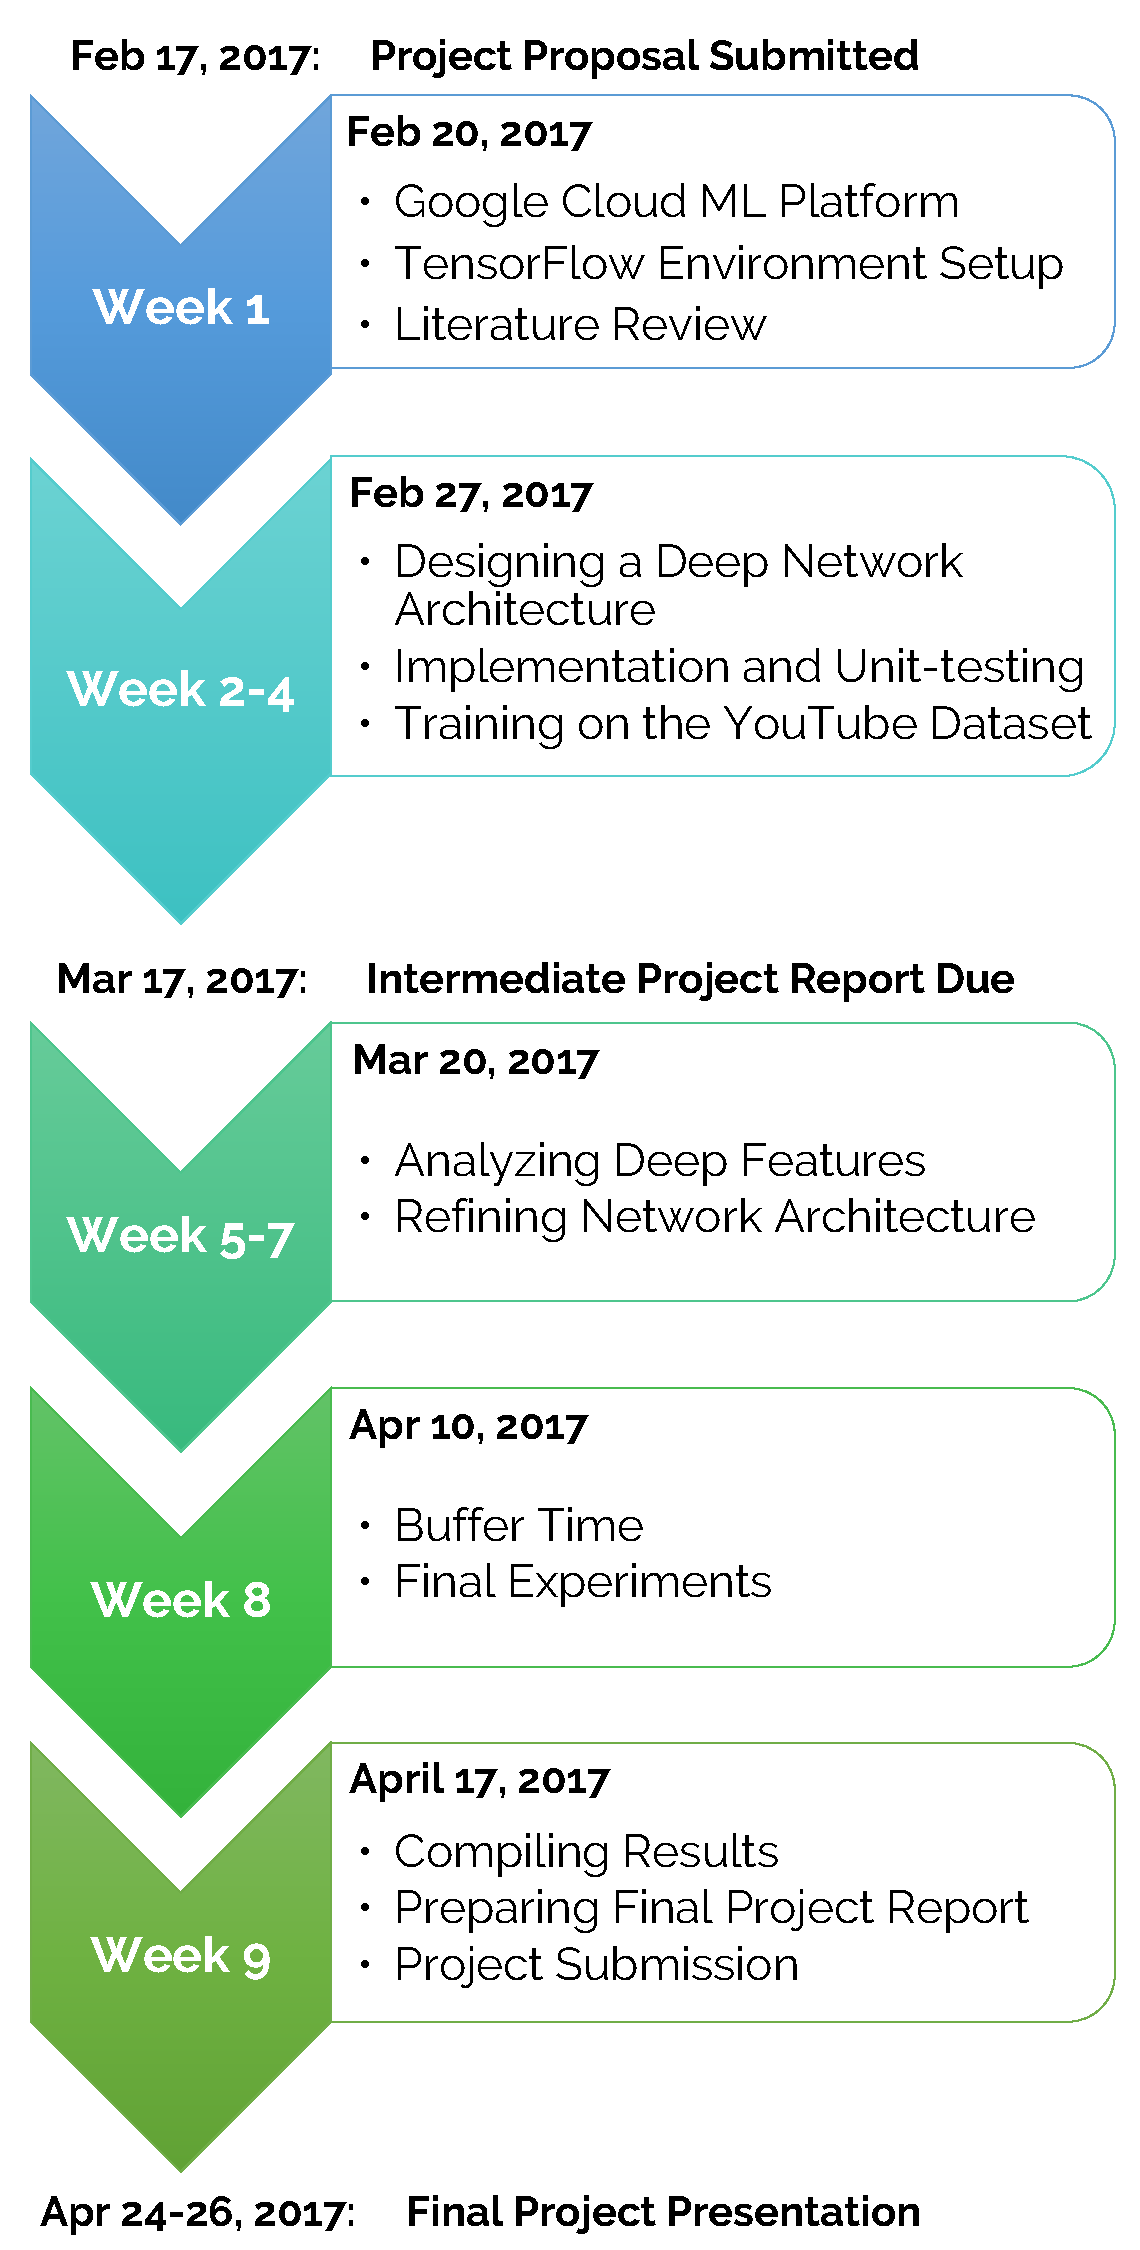
\includegraphics[width=0.85\linewidth]{timeline.pdf}
    \caption{Timeline presenting the targeted milestones in the project.}
    \label{fig:timeline}
\end{figure}

\section{Project Timeline}
The first milestone for us is to prepare ourselves for this challenging task. It is crucial to perform a comprehensive literature review to understand the existing methodology and algorithms, and understand their strengths and weaknesses. We will primarily focus on the studies based on deep learning. We will also get acquainted with the Google Cloud Machine Learning platform and setup the required environment to use TensorFlow. We have allotted 1 full week for this task, which also includes a buffer time if we face any challenges in getting used to the new environment.

The next milestone for us it to implement our understanding. This will include design, implementation and training of a deep neural network architecture. We also plan to put sufficient time in getting acquainted with the YouTube dataset.
	
Once we obtain a preliminary set of results, we will spend time to understand the limitations of our architecture and refining it. This will include parameter and architecture tuning using cross-validation. We also plan to analyze the deep features learnt by the network, to improve our understanding and take steps towards improving the overall performance.
	
Lastly, we will run the final set of experiments and compile the results to prepare for our final project report and presentation. Figure \ref{fig:timeline} shows the overview of our project timeline.




\bibliographystyle{unsrt}
\bibliography{ml_bib}  

\end{document}
